\chapter[Result and Analysis]{Result and Analysis}
\markboth{Chap. 3\ \ \enspace Experimental methods}{Chap 2. Experimental methods}

\regularsection
\headerregularsection

\updatemylof % to be used with "list of figure divider per chapter" (see PREAMBLE)
\updatemylot % to be used with "list of table divider per chapter" (see PREAMBLE)

\begin{sloppypar} % to suppress overfull box
Here we will compare our model with existing models and our proposed model result. We tried this dataset in 5 different models: 
\end{sloppypar}



\begin{table}[!h]
  \centering
  \caption[YOLO Network Structure]{YOLO Network Structure}
  \label{tab:yolo-network}
  {\renewcommand{\arraystretch}{1.7}
      \begin{tabular}{p{4cm} p{1cm} p{0.8cm} p{1cm} p{2.6cm}}
          \toprule
          Model Name                                    & mAP (our dataset) & COCO mAP & Speed (ms) & Detect Small object and less overlapping \\
          \hline
          EfficientDet D4 1024x1024                     & 12.27             & 48.5     & 133        & YES                                      \\
          SSD ResNet152 V1 FPN 1024x1024 (RetinaNet152) & 8.75              & 38.3     & 104        & NO                                       \\
          Faster R-CNN ResNet101 V1 1024x1024           & 11.56             & 37.1     & 72         & NO                                       \\
          Faster R-CNN Inception ResNet V2 1024x1024    & 11.89             & 38.7     & 236        & NO                                       \\
          YOLO v5(1024x1024)                            & 12.06             & 49.7     & 65         & YES                                      \\
          YOLO v5(1024x1024) Modified (Proposed Method) & 13.46             & 49.8     & 70         & YES                                      \\
          \bottomrule
    \end{tabular}
  }
\end{table}

After benchmarking with above model we found that our model do best both in time and accuracy.

The dataset in the start is labelled for 21 classes {Ambulance, Auto Rickshaw, Bicycle, Bus, Car, Garbage Van, Human Hauler, Minibus, Minivan, Motorbike, Pickup, Army Vehicle, Police Car, Rickshaw, Scooter, SUV, Taxi, Three Wheelers (CNG), Truck, Van, Wheelbarrow} and has been trained for 60 epochs using the network configuration of~\ref{tab:yolo-parameter}.  The  network  has been  trained  for  60  epochs  that  are  20000  iterations  (4 epochs  are
1328 iterations) because darknet framework trains a maximum of 2000 iterations for each class
and calculates the mAP@0.5 every 4 epochs for the validation set and every 3 epochs for the
test set unless the difference between the cost of an iteration and the cost of the next iteration
is lower than 0.0005.


\begin{table}[!h]
  \centering
  \caption[Initial values for the YOLO network parameters.]{Initial values for the YOLO network parameters.}
  \label{tab:yolo-parameter}
  {\renewcommand{\arraystretch}{1.7}
    \begin{tabular}{p{6.5cm} p{4cm}}
          \toprule
          Parameter                                                                         & Value  \\
          \hline
          Batch size                                                                        & 64 \\ 
          Subdivisions = sub batches: number of mini batches it is split up the batch       & 32 \\
          Width $\times$ height of the input images                                         & 416 $\times$ 416  \\
          IoU minimum threshold between predicted BB and ground-truth                       & 0.5 \\
          Data augmentation                                                                 & Saturation and exposure=1.5 angle=0 hue=0.1  \\
          Learning rate                                                                     & 0.001 \\
          Max\_batches                                                                      & Number class $\times$ 2000 \\
          Momentum                                                                          & 0.9 \\
          Decay                                                                             & 0.0005 \\
          \bottomrule
    \end{tabular}
  }
\end{table}

\begin{table}[!h]
  \centering
  \caption[Evaluation of the model]{Evaluation of the model on the validation set with an IoU threshold of 50% that is the 
Area-Under-Curve for each unique Recall. }
  \label{tab:class-ap}
  {\renewcommand{\arraystretch}{1.7}
    \begin{tabular}{p{1.5cm} p{1.5cm} p{1.5cm} p{1.5cm} p{1.5cm} p{1.5cm}}
          \toprule
          Epochs & Ap Car & Ap Rickshaw & Ap  Bus & Ap SUV & Ap Truck \\
          \hline
          3 & 39.35\% & 09.33\% & 39.57\% & 16.76\% & 27.82\% \\
          6 & 41.65\% & 13.68\% & 41.73\% & 18.74\% & 30.76\% \\ 
          9 & 44.15\% & 15.01\% & 43.53\% & 19.02\% & 32.07\% \\
          12 & 48.35\% & 15.93\% & 46.98\% & 19.38\% & 33.43\% \\
          15 & 49.89\% & 16.45\% & 50.13\% & 20.31\% & 34.76\% \\
          \bottomrule
    \end{tabular}
  }
\end{table}

For evaluating which weight file is the best one to use for detecting vehicles in new images we 
will guide by the mAP value computed in the validation and test set. In the~\ref{tab:class-ap} we can 
see which weights files give best value on the mAP. The training has been done for 15 epochs, 
but  it  can  happen  that  the  weights  computed  in  previous  epochs  give  a  better  value  on  the 
precision and the mAP. This may happen due to overfitting; the model is very good detecting on 
the training set but falls to detect objects in new images. As it can be seen in Table 4, the weight 
file  stored in the epoch 15 and the epoch 18 obtain the  best mAP value of 37.20\% and in the 
Table 3 the weight file obtained in the epoch 16 gets a 35.52\% mAP best value.  

%\begin{figure}[H] % \begin{figure}[H] for forcing the figure placement here ; in the bottom, \begin{figure}[!b] ; top of the page, \begin{figure}[!t] ; otherwise, \begin{figure} will let LaTeX decide the best figure placement for you
%    \begin{minipage}{0.45\textwidth}
%  \centering
%  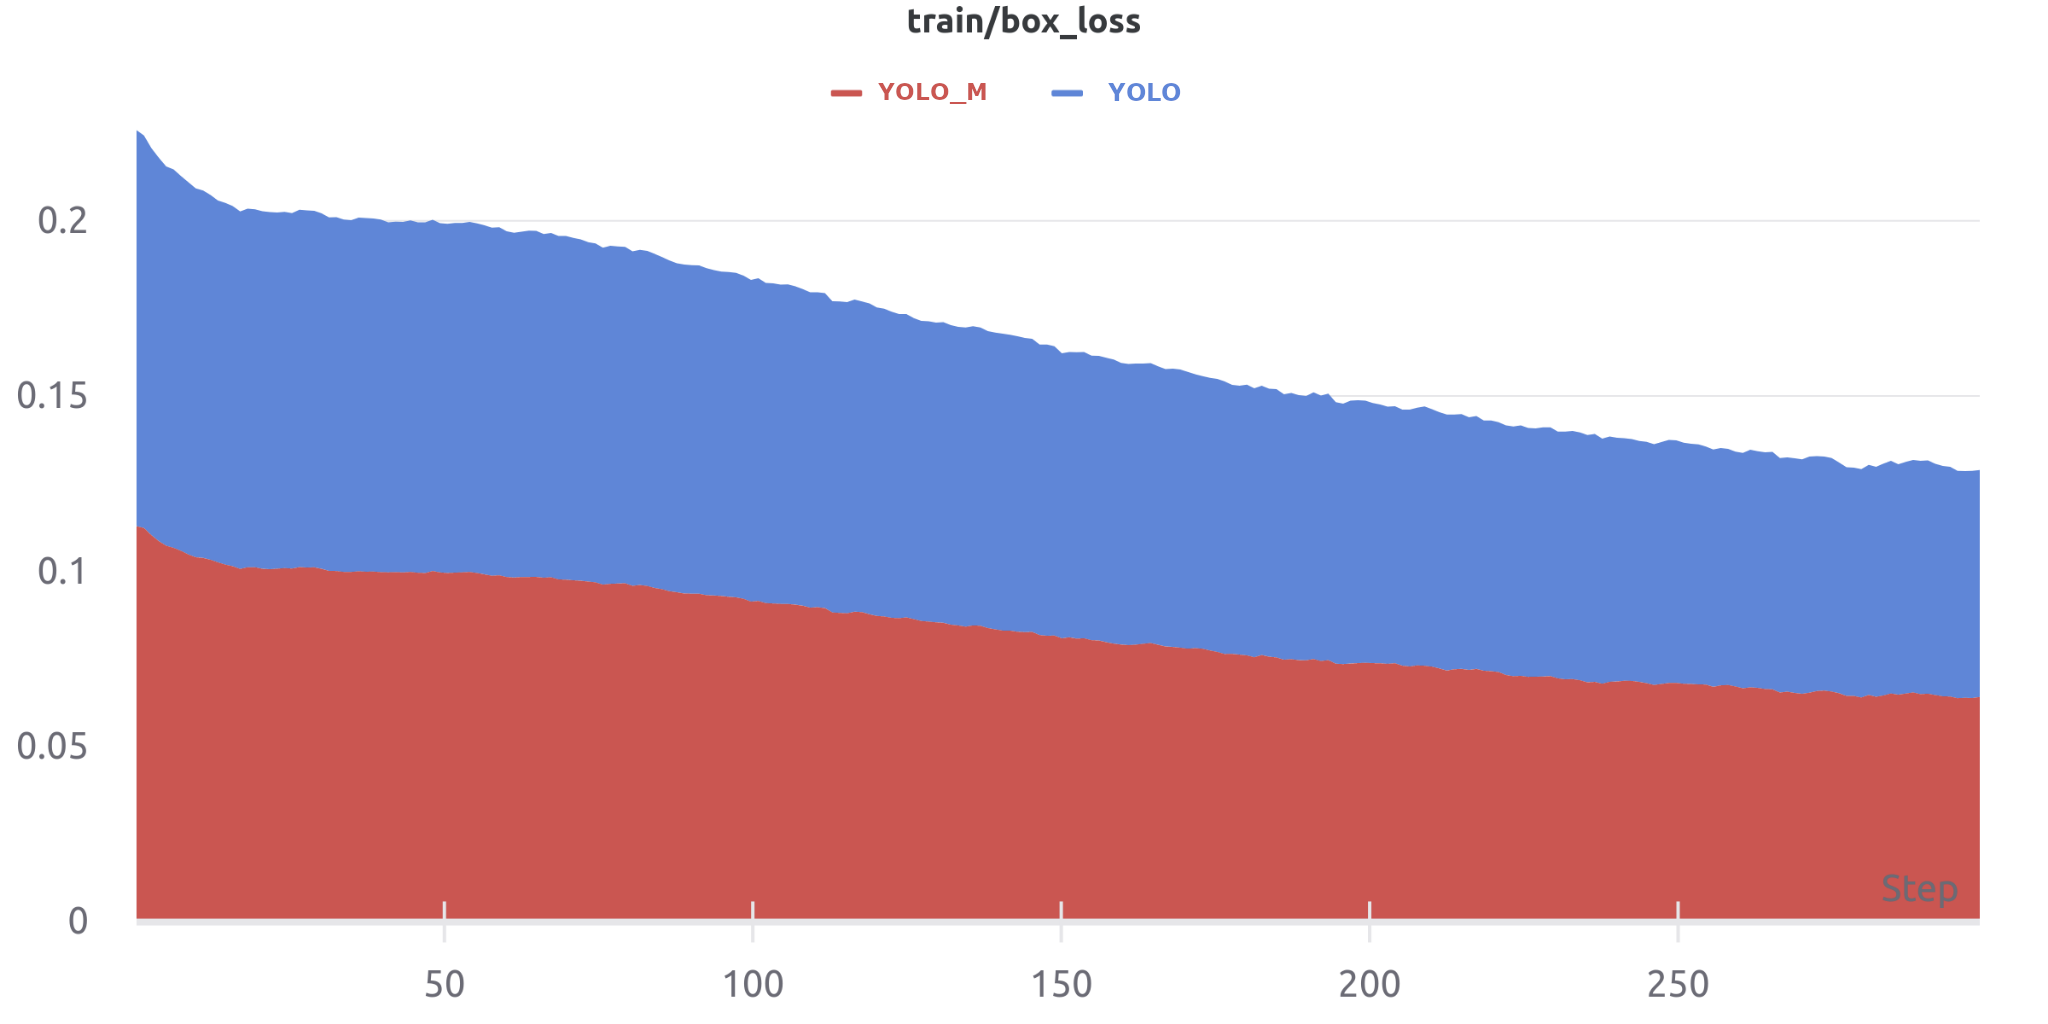
\includegraphics[width=0.9\textwidth]{figures/paper/box-loss.png}
%  \caption[The Architecture]{\textbf{The Architecture}. }
%  \label{fig:figures/paper/box-loss}
%  \end{minipage}\hfill
%%\end{figure}


%%\begin{figure}[H] % \begin{figure}[H] for forcing the figure placement here ; in the bottom, \begin{figure}[!b] ; top of the page, \begin{figure}[!t] ; otherwise, \begin{figure} will let LaTeX decide the best figure placement for you
%  \begin{minipage}{0.45\textwidth}
%  \centering
%  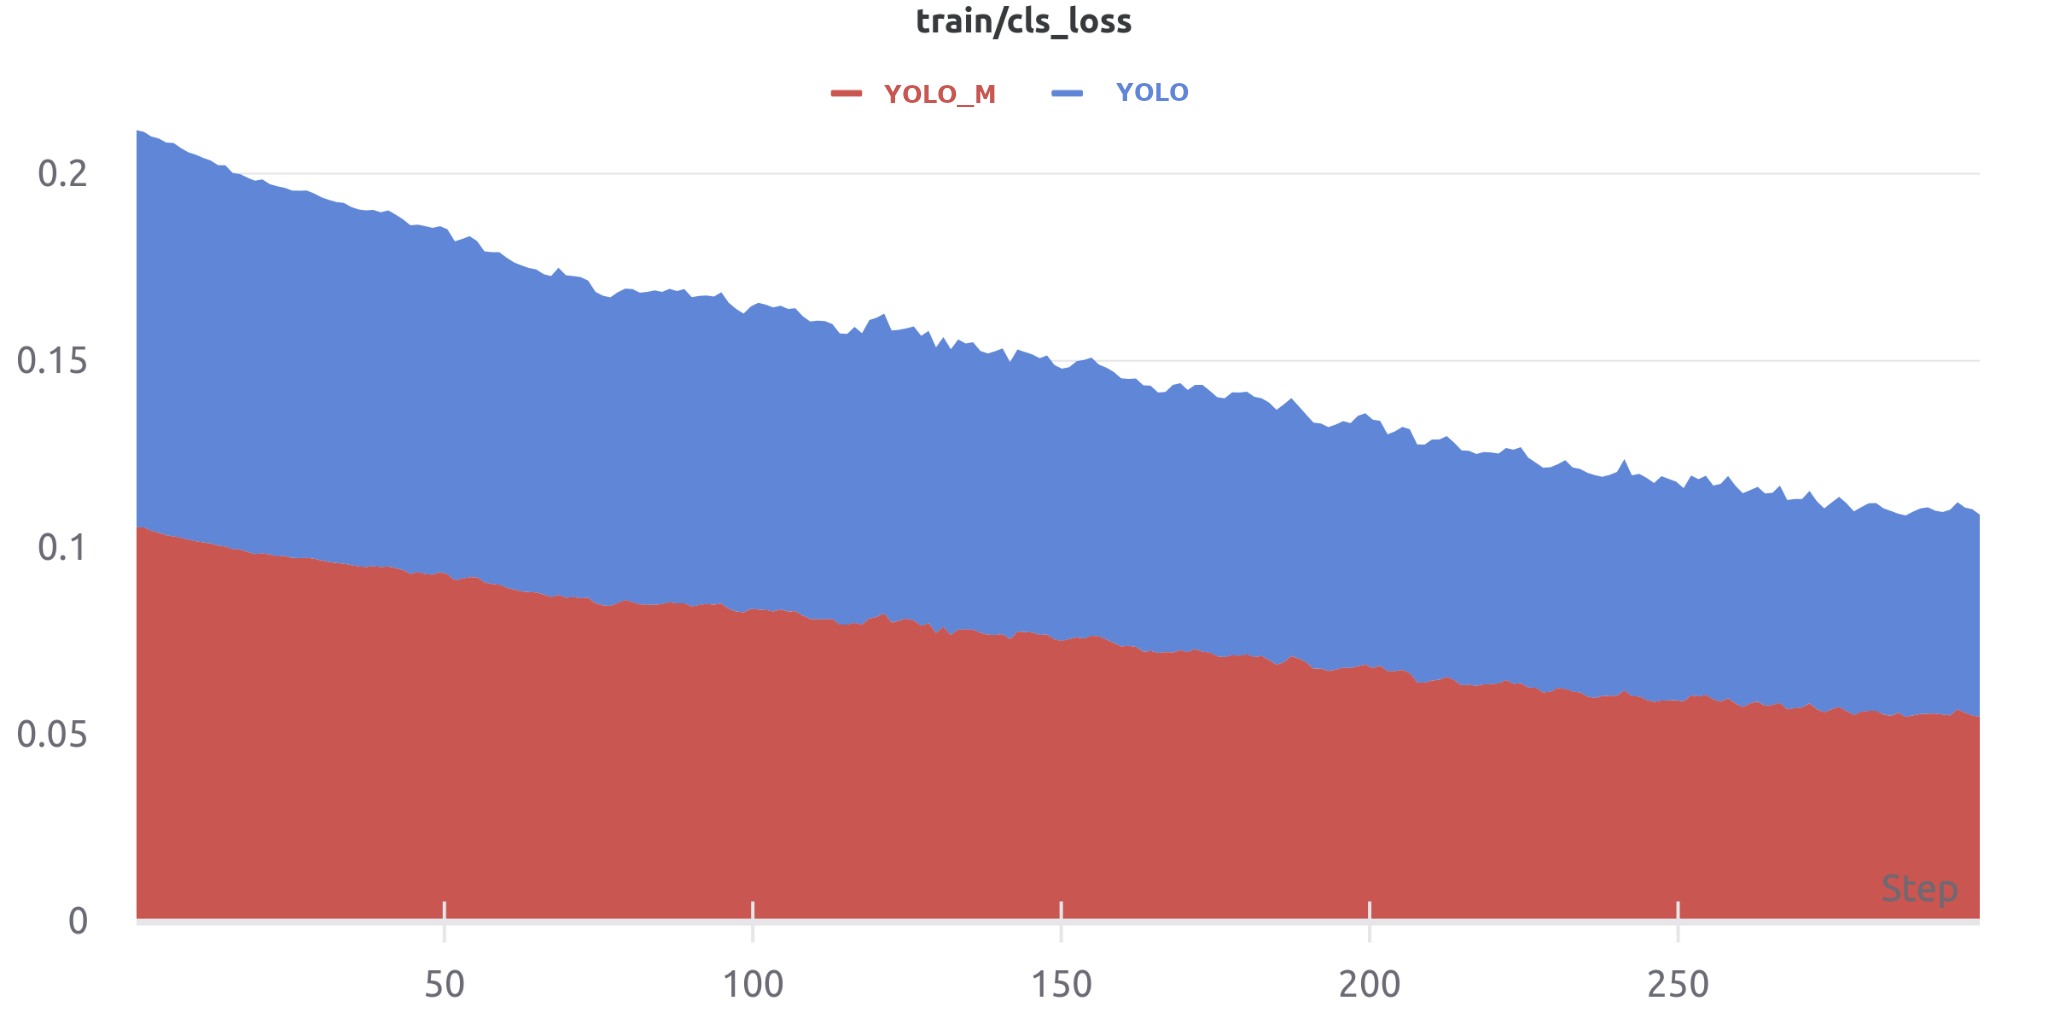
\includegraphics[width=0.9\textwidth]{figures/paper/cls-loss.png}
%  \caption[The Architecture]{\textbf{The Architecture}. }
%  \label{fig:figures/paper/cls-loss}
%  \end{minipage}
%\end{figure}


\begin{figure}
    \centering
    \begin{minipage}{0.48\textwidth}
        \centering
  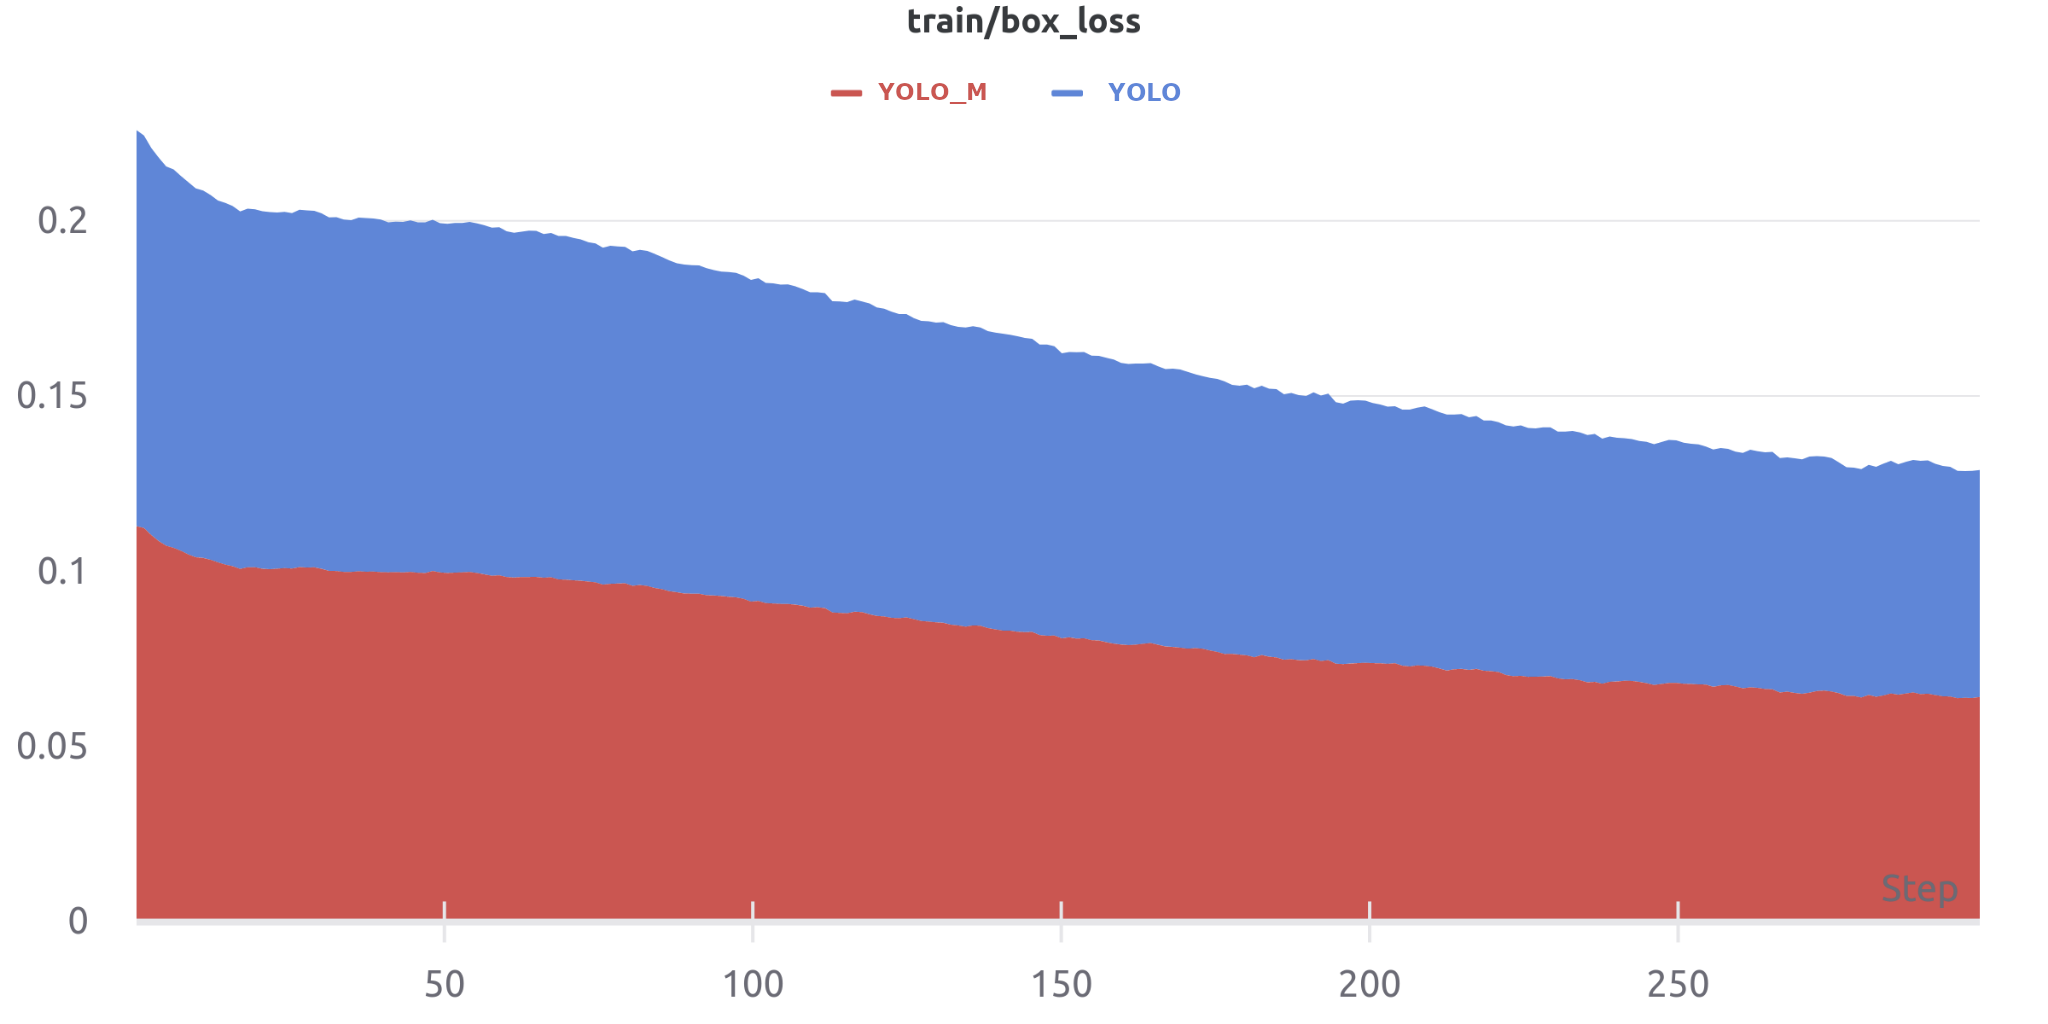
\includegraphics[width=\textwidth]{figures/paper/box-loss.png}
    \end{minipage}\hfill
    \begin{minipage}{0.48\textwidth}
        \centering
  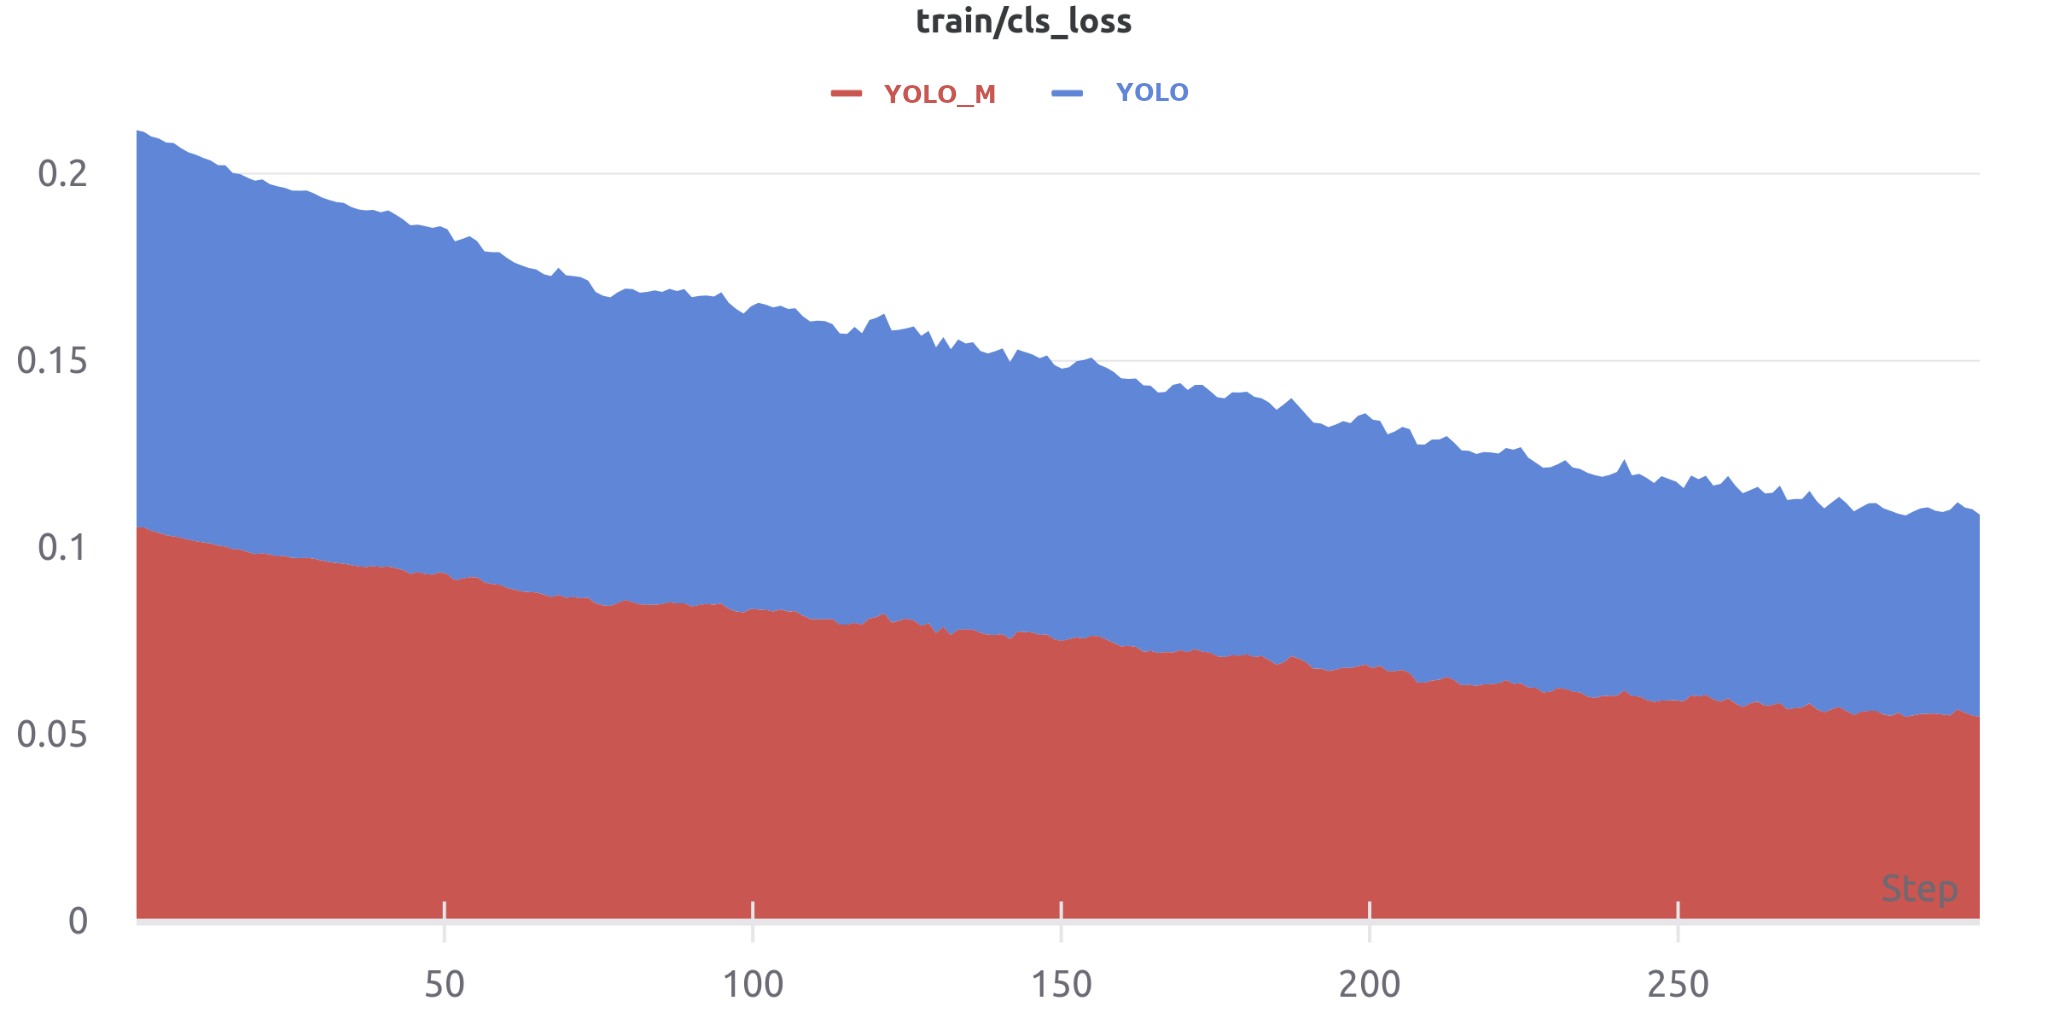
\includegraphics[width=\textwidth]{figures/paper/cls-loss.png}
    \end{minipage}
    \caption[Box loss and Classificaton loss]{\textbf{Losses over Epochs} Box loss and Classificaton loss }
  \label{fig:figures/paper/box-loss}
\end{figure}






\begin{figure}[H] % \begin{figure}[H] for forcing the figure placement here ; in the bottom, \begin{figure}[!b] ; top of the page, \begin{figure}[!t] ; otherwise, \begin{figure} will let LaTeX decide the best figure placement for you
  \centering
  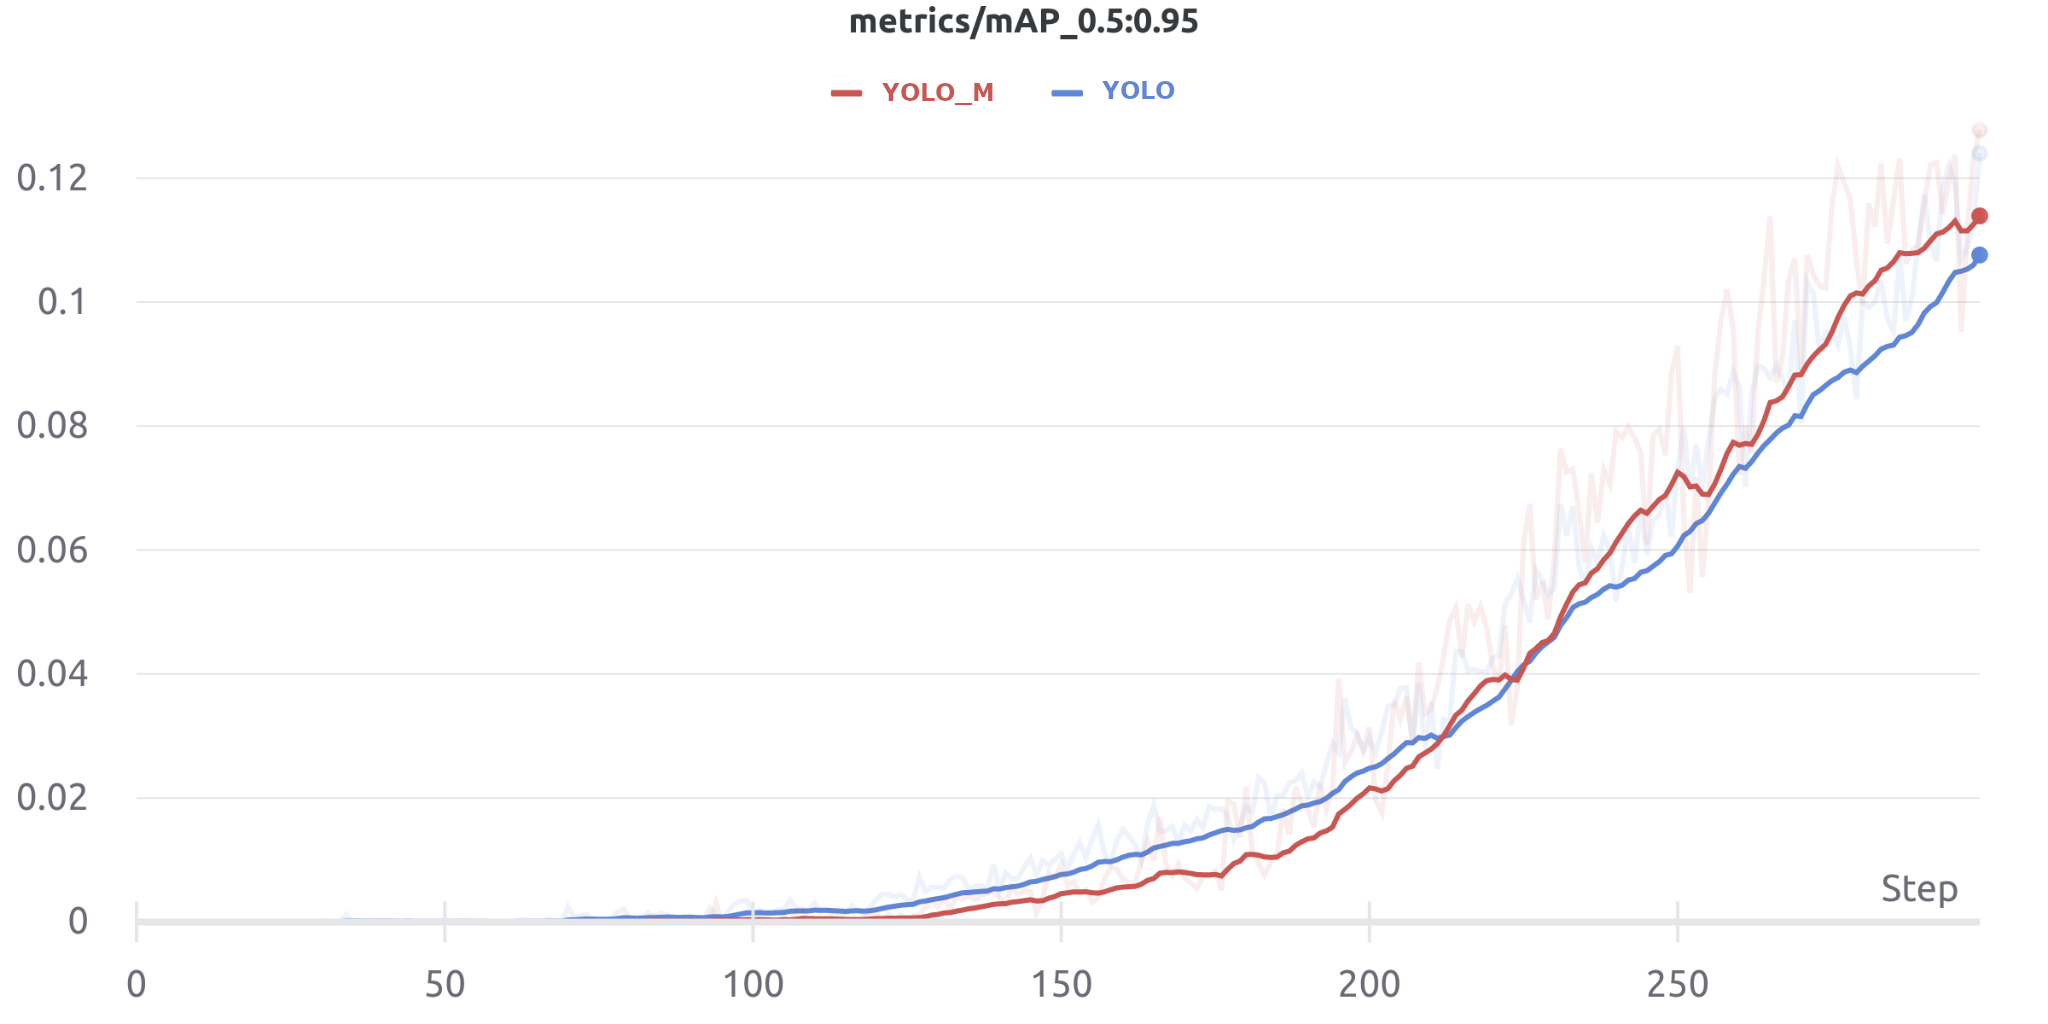
\includegraphics[width=\textwidth]{figures/paper/mAP.png}
  \caption[The Architecture]{\textbf{mAP Comparison of YOLOv5 and Modified YOLO with ORB}. Graph computed during the training; the mAP is computed over the validation set.}
  \label{fig:figures/paper/mAP}
\end{figure}

In the~\ref{fig:figures/paper/mAP} we can see the graph that shows the average loss computed for every iteration
and  the  mAP  calculated  for  every  4  epochs  (1  epoch  =  332  iterations  so  4  epochs  =  1328
iterations). The value of the  loss remains between 3.5 and 4  and the mAP has a value of 35\%
from the iteration 5000 (epoch 15) to the iteration 6000 (epoch 18). With the~\ref{fig:figures/paper/mAP}
and the~\ref{tab:class-ap} we can conclude that the best weight file for detecting vehicles in new
images is obtained in the epoch 15. Note that the dataset is quite complex as it has many
labelled small vehicles in each images that are not visually easy to see, this complexity affects
the mAP value by obtaining a relatively low one. This happens because the model fails to detect
some vehicles in the validation set that it is difficult even for the human eye to detect them. On
the next pages, to test the capability of generalizing of our model for this training, we will get
one image containing cars, other image containing trucks, other image containing motors and a
final image containing cars, trucks and SUVs and pass them from our model to see if it is able
to detect all the vehicles in the images.



\begin{figure}[H] % \begin{figure}[H] for forcing the figure placement here ; in the bottom, \begin{figure}[!b] ; top of the page, \begin{figure}[!t] ; otherwise, \begin{figure} will let LaTeX decide the best figure placement for you
  \centering
  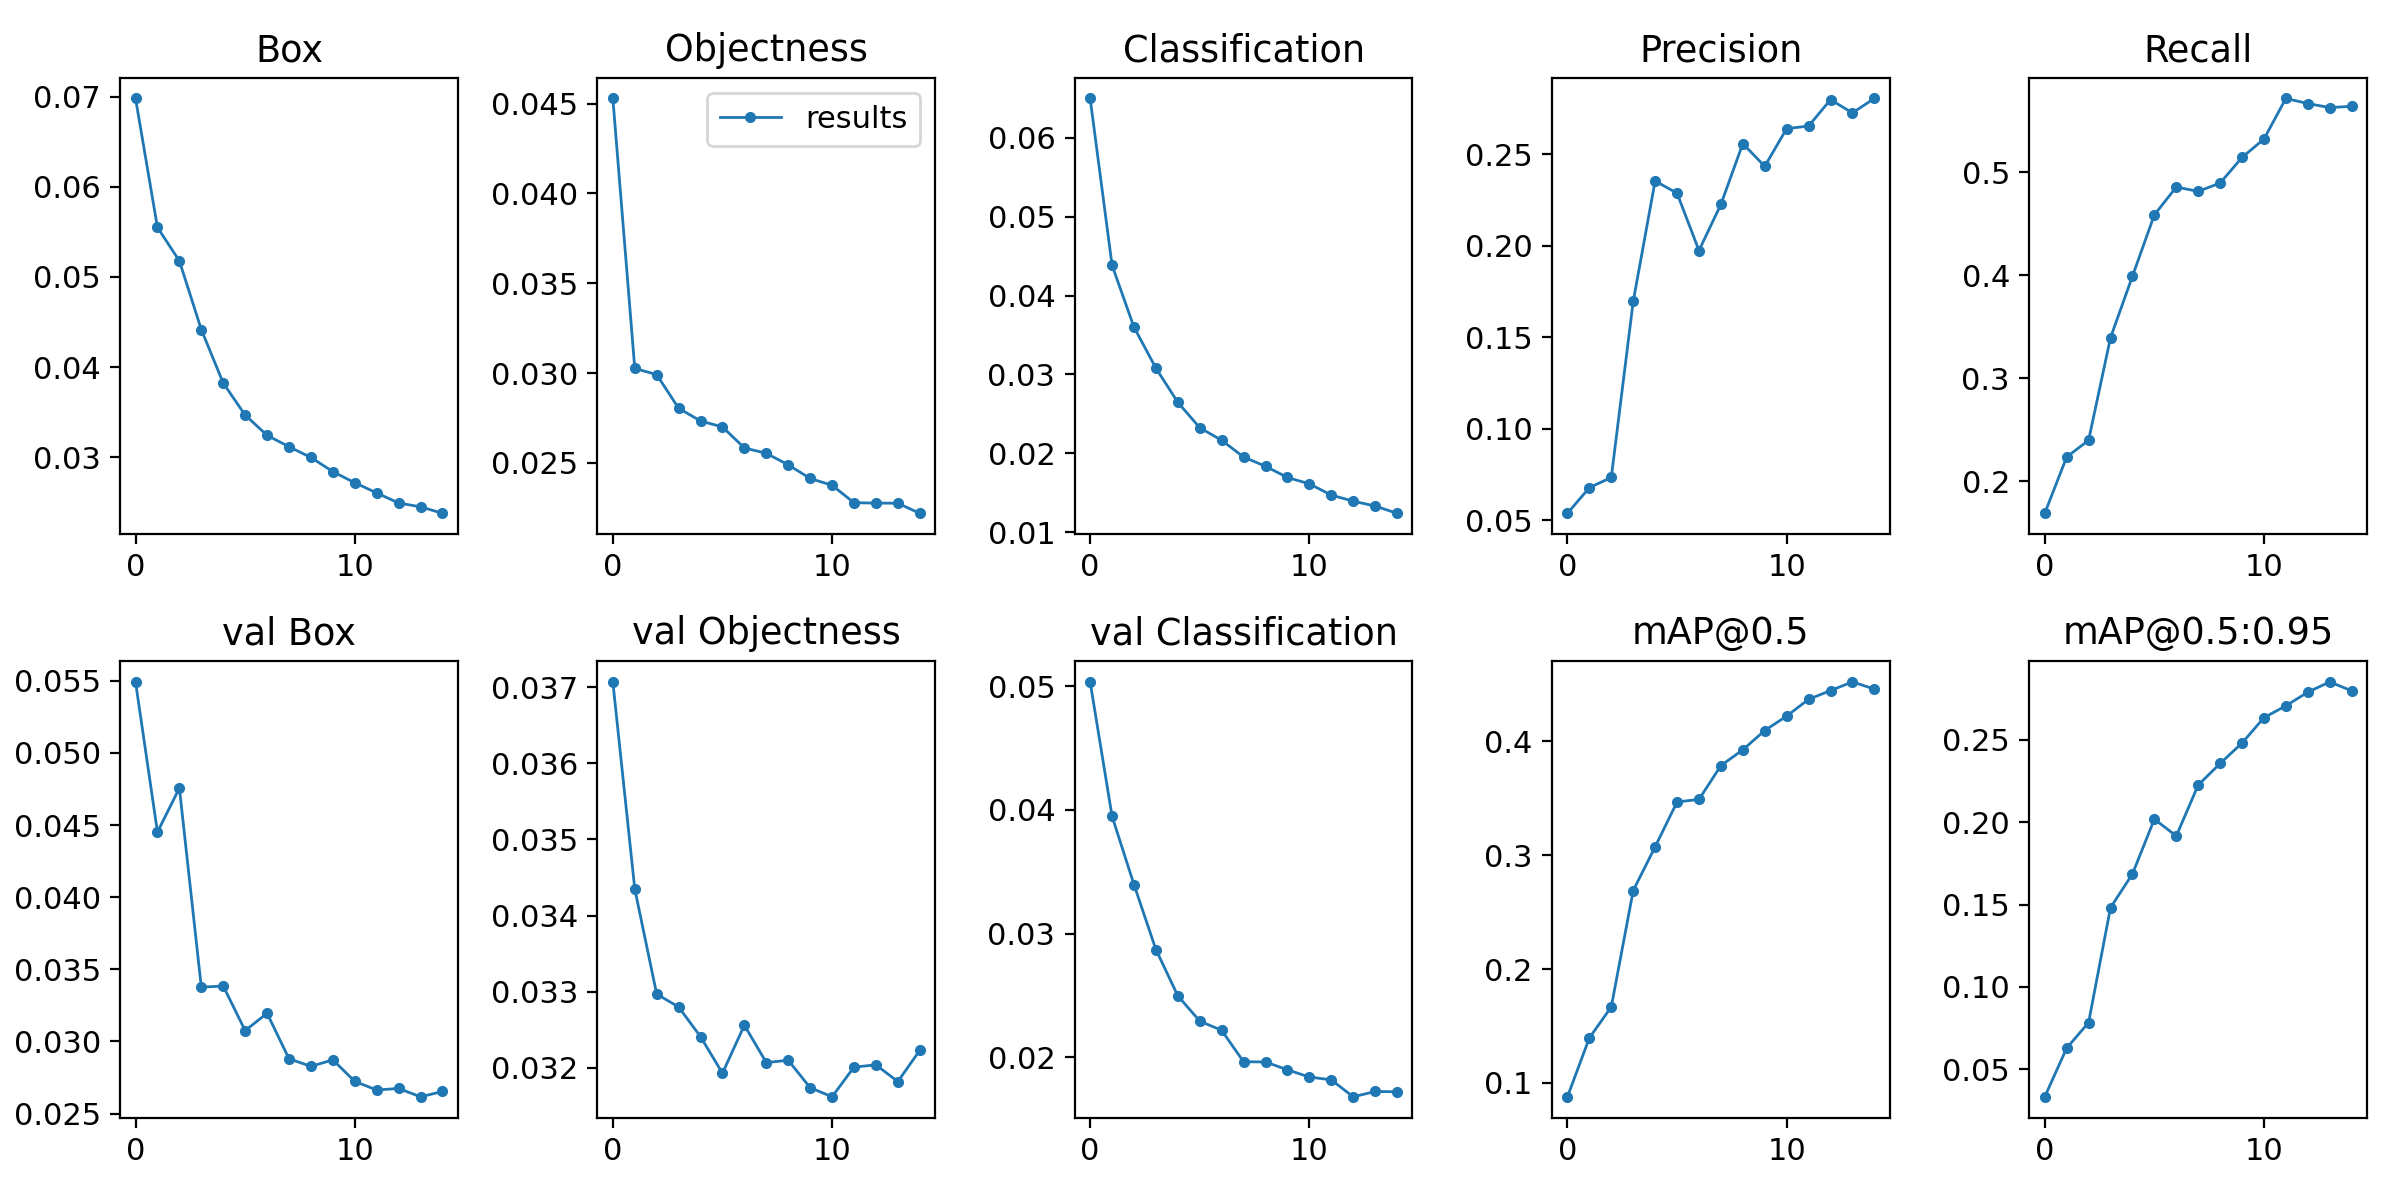
\includegraphics[width=\textwidth]{figures/paper/results.png}
  \caption[The Architecture]{\textbf{Result of Dhaka AI and Indian Driving Dataset}. }
  \label{fig:figures/paper/results}
\end{figure}

\begin{figure}[H] % \begin{figure}[H] for forcing the figure placement here ; in the bottom, \begin{figure}[!b] ; top of the page, \begin{figure}[!t] ; otherwise, \begin{figure} will let LaTeX decide the best figure placement for you
  \centering
  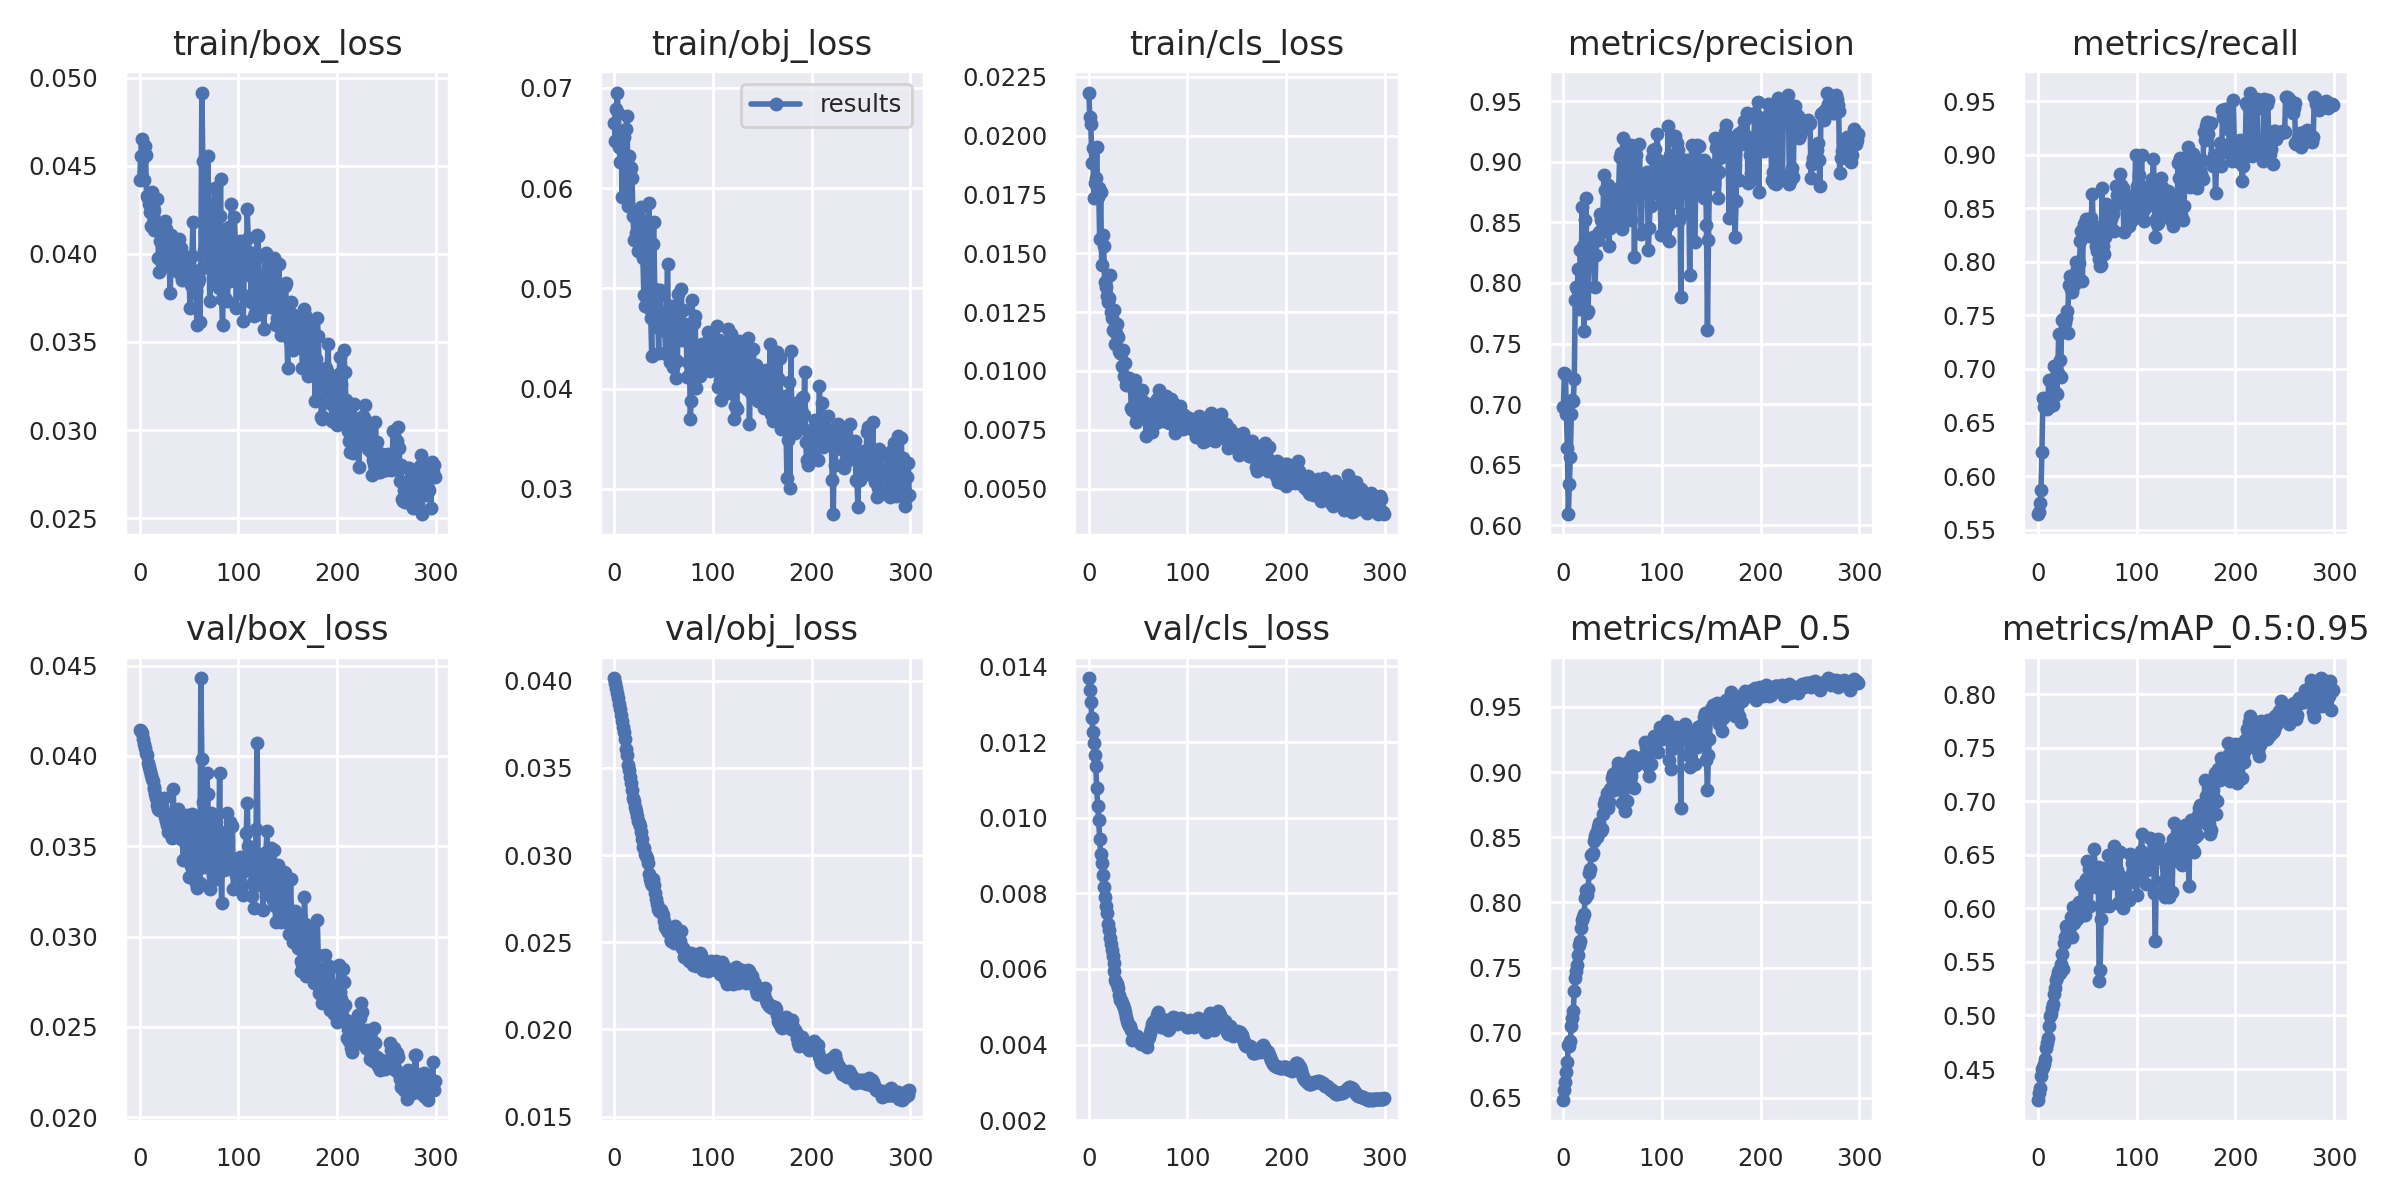
\includegraphics[width=\textwidth]{figures/paper/yolo-on-coco.png}
  \caption[The Architecture]{\textbf{Result on COCO}. }
  \label{fig:figures/paper/yolo-on-coco}
\end{figure}


%=======================================================================
%%% References

% \clearpage
\phantomsection
\specialsection % put an indent, see preamble
\headerspecialsection

{\hypersetup{urlcolor=ntnu,linkcolor=sophia} % set clickable URL title color to black, not ntnu like in the main document

  \bibliographystyle{unsrtnat-mod}  % NATBIB ref style
  \bibliography{references}
}
